%%% Local Variables:
%%% mode: latex
%%% TeX-master: t
%%% End:

%\documentclass[bachelor,nofonts]{thuthesis}
\documentclass[master]{thuthesis}
%\documentclass[doctor]{thuthesis}
% \documentclass[%
%   bachelor|master|doctor|postdoctor, % mandatory option
%   winfonts|nofonts|adobefonts, % mandatory only for bachelor and Linuxer
%   secret,
%   openany|openright,
%   arialtoc,arialtitle]{thuthesis}
% 当使用 XeLaTeX 编译时,本科生、Linux 用户需要加上 nofonts 选项;
% 当使用 PDFLaTeX 编译时,adobefonts 选项等效于 winfonts 选项(缺省选项)。

% 所有其它可能用到的包都统一放到这里了,可以根据自己的实际添加或者删除。
\usepackage{thutils}
\usepackage{lineno,hyperref}
% 你可以在这里修改配置文件中的定义,导言区可以使用中文。
% \def\myname{薛瑞尼}
\usepackage{amsmath}
\usepackage{comment}
\usepackage{algorithm}
\usepackage{algorithmic}
\usepackage{setspace}
\begin{document}

% 定义所有的eps文件在 figures 子目录下
\graphicspath{{figures/}}


%%% 封面部分
\frontmatter

%%% Local Variables:
%%% mode: latex
%%% TeX-master: t
%%% End:

% 中国海洋大学研究生学位论文封面
% 参考:中国海洋大学研究生学位论文书写格式20130307.doc

% 为避免出现错误,下面保留[清华大学学位论文模板原有定义无需修改],
% 请直接跳到后面[中国海洋大学学位论文模板部分请根据自己情况修改]。

%%%%%%%%%%%%%%%%%%%%%%[清华大学学位论文模板原有定义无需修改]%%%%%%%%%%%%%%%%%%%%%%%
\secretlevel{绝密} \secretyear{2100}

\ctitle{清华大学学位论文 \LaTeX\ 模板\\使用示例文档}
% 根据自己的情况选,不用这样复杂
\makeatletter
\ifthu@bachelor\relax\else
  \ifthu@doctor
    \cdegree{工学博士}
  \else
    \ifthu@master
      \cdegree{工学硕士}
    \fi
  \fi
\fi
\makeatother


\cdepartment[计算机]{计算机科学与技术系}
\cmajor{计算机科学与技术}
\cauthor{薛瑞尼} 
\csupervisor{郑纬民教授}
% 如果没有副指导老师或者联合指导老师,把下面两行相应的删除即可。
\cassosupervisor{陈文光教授}
\ccosupervisor{某某某教授}
% 日期自动生成,如果你要自己写就改这个cdate
%\cdate{\CJKdigits{\the\year}年\CJKnumber{\the\month}月}

% 博士后部分
% \cfirstdiscipline{计算机科学与技术}
% \cseconddiscipline{系统结构}
% \postdoctordate{2009年7月——2011年7月}

\etitle{An Introduction to \LaTeX{} Thesis Template of Tsinghua University} 
% 这块比较复杂,需要分情况讨论:
% 1. 学术型硕士
%    \edegree:必须为Master of Arts或Master of Science(注意大小写)
%              “哲学、文学、历史学、法学、教育学、艺术学门类,公共管理学科
%               填写Master of Arts,其它填写Master of Science”
%    \emajor:“获得一级学科授权的学科填写一级学科名称,其它填写二级学科名称”
% 2. 专业型硕士
%    \edegree:“填写专业学位英文名称全称”
%    \emajor:“工程硕士填写工程领域,其它专业学位不填写此项”
% 3. 学术型博士
%    \edegree:Doctor of Philosophy(注意大小写)
%    \emajor:“获得一级学科授权的学科填写一级学科名称,其它填写二级学科名称”
% 4. 专业型博士
%    \edegree:“填写专业学位英文名称全称”
%    \emajor:不填写此项
\edegree{Doctor of Engineering} 
\emajor{Computer Science and Technology} 
\eauthor{Xue Ruini} 
\esupervisor{Professor Zheng Weimin} 
\eassosupervisor{Chen Wenguang} 
% 这个日期也会自动生成,你要改么?
% \edate{December, 2005}

% 定义中英文摘要和关键字
\begin{cabstract}
  论文的摘要是对论文研究内容和成果的高度概括。摘要应对论文所研究的问题及其研究目
  的进行描述,对研究方法和过程进行简单介绍,对研究成果和所得结论进行概括。摘要应
  具有独立性和自明性,其内容应包含与论文全文同等量的主要信息。使读者即使不阅读全
  文,通过摘要就能了解论文的总体内容和主要成果。

  论文摘要的书写应力求精确、简明。切忌写成对论文书写内容进行提要的形式,尤其要避
  免“第 1 章……;第 2 章……;……”这种或类似的陈述方式。

  本文介绍清华大学论文模板 \thuthesis{} 的使用方法。本模板符合学校的本科、硕士、
  博士论文格式要求。

  本文的创新点主要有:
  \begin{itemize}
    \item 用例子来解释模板的使用方法;
    \item 用废话来填充无关紧要的部分;
    \item 一边学习摸索一边编写新代码。
  \end{itemize}

  关键词是为了文献标引工作、用以表示全文主要内容信息的单词或术语。关键词不超过 5
  个,每个关键词中间用分号分隔。(模板作者注:关键词分隔符不用考虑,模板会自动处
  理。英文关键词同理。)
\end{cabstract}

\ckeywords{\TeX, \LaTeX, CJK, 模板, 论文}

\begin{eabstract} 
   An abstract of a dissertation is a summary and extraction of research work
   and contributions. Included in an abstract should be description of research
   topic and research objective, brief introduction to methodology and research
   process, and summarization of conclusion and contributions of the
   research. An abstract should be characterized by independence and clarity and
   carry identical information with the dissertation. It should be such that the
   general idea and major contributions of the dissertation are conveyed without
   reading the dissertation. 

   An abstract should be concise and to the point. It is a misunderstanding to
   make an abstract an outline of the dissertation and words ``the first
   chapter'', ``the second chapter'' and the like should be avoided in the
   abstract.

   Key words are terms used in a dissertation for indexing, reflecting core
   information of the dissertation. An abstract may contain a maximum of 5 key
   words, with semi-colons used in between to separate one another.
\end{eabstract}

\ekeywords{\TeX, \LaTeX, CJK, template, thesis}
%%%%%%%%%%%%%%%%%%%%%%%%%%%%%%%%%%%%%%%%%%%%%%%%%%%%%%%%%%%%%%%%%%%%%%%%%%%%%%%%

%%%%%%%%%%%%%%%%%%[中国海洋大学学位论文模板部分请根据自己情况修改]%%%%%%%%%%%%%%%%%%%
% 中国海洋大学研究生学位论文封面
% 必须填写的内容包括(其他最好不要修改):
%   分类号、密级、UDC
%   论文中文题目、作者中文姓名
%   论文答辩时间
%   封面感谢语
%   论文英文题目
%   中文摘要、中文关键词
%   英文摘要、英文关键词
%
%%%%%[自定义]%%%%%
\newcommand{\fenleihao}{}%分类号
\newcommand{\miji}{}%密级 
                    % 绝密$\bigstar$20年 
                    % 机密$\bigstar$10年
                    % 秘密$\bigstar$5年
\newcommand{\UDC}{}%UDC
\newcommand{\oucctitle}{角毛藻显微图像分割}%论文中文题目
\ctitle{角毛藻显微图像分割}%必须修改因为页眉中用到
\cauthor{***}%可以选择修改因为仅在 pdf 文档信息中用到
\cdegree{工学}%可以选择修改因为仅在 pdf 文档信息中用到
\ckeywords{\TeX, \LaTeX, CJK, 模板, 论文}%可以选择修改因为仅在 pdf 文档信息中用到
\newcommand{\ouccauthor}{汤宁}%作者中文姓名
%\newcommand{\ouccauthor}{***}%外审时用到
%\newcommand{\ouccsupervisor}{姬光荣教授}%作者导师中文姓名
%\newcommand{\ouccdegree}{博\hspace{1em}士}%作者申请学位级别
%\newcommand{\ouccmajor}{海洋信息探测与处理}%作者专业名称
%\newcommand{\ouccdateday}{\CJKdigits{\the\year}年\CJKnumber{\the\month}月\CJKnumber{\the\day}日}
%\newcommand{\ouccdate}{\CJKdigits{\the\year}年\CJKnumber{\the\month}月}
\newcommand{\oucdatedefense}{           }%论文答辩时间
%\newcommand{\oucdatedegree}{2009年6月}%学位授予时间
\newcommand{\oucgratitude}{谨以此论文献给我的导师和亲人!}%封面感谢语
\newcommand{\oucetitle}{\emph{Chaetoceros} Microscopic Image Segmentation}%论文英文题目
%\newcommand{\ouceauthor}{Haiyong Zheng}%作者英文姓名
\newcommand{\oucthesis}{\textsc{OUCThesis}}
%%%%%默认自定义命令%%%%%
% 空下划线定义
\newcommand{\oucblankunderline}[1]{\rule[-2pt]{#1}{.7pt}}
\newcommand{\oucunderline}[2]{\underline{\hskip #1 #2 \hskip#1}}

% 论文封面第一页
%%不需要改动%%
\vspace*{5cm}
{\xiaoer\heiti\oucgratitude

\begin{flushright}
---\hspace*{-2mm}---\hspace*{-2mm}---\hspace*{-2mm}---\hspace*{-2mm}---\hspace*{-2mm}---\hspace*{-2mm}---\hspace*{-2mm}---\hspace*{-2mm}---\hspace*{-2mm}---~\ouccauthor
\end{flushright}
}

%\begin{comment}

\newpage 
%\mbox{} 
%\newpage

% 论文封面第二页
%%不需要改动%%
\vspace*{1cm}
\begin{center}
  {\xiaoer\heiti\oucctitle}
\end{center}
\vspace{10.7cm}
{\normalsize\songti
\begin{flushright}
{\renewcommand{\arraystretch}{1.3}
  \begin{tabular}{r@{}l}
    学位论文答辩日期:~ & \oucunderline{2.5cm}{\oucdatedefense} \\
    指导教师签字:~ & \oucblankunderline{5cm} \\
    答辩委员会成员签字:~ & \oucblankunderline{5cm} \\
    ~ & \oucblankunderline{5cm} \\
    ~ & \oucblankunderline{5cm} \\
    ~ & \oucblankunderline{5cm} \\
    ~ & \oucblankunderline{5cm} \\
    ~ & \oucblankunderline{5cm} \\
    ~ & \oucblankunderline{5cm} \\
  \end{tabular}
}
\end{flushright}
}



\newpage 
%\mbox{} 
%\newpage

\pagestyle{plain}
\clearpage\pagenumbering{roman}

% 中文摘要
%%[需要填写:中文摘要、中文关键词]%%
\begin{center}
  {\sanhao[1.5]\heiti\oucctitle\\\vskip7pt 摘\hspace{1em}要}
\end{center}
{\normalsize\songti

  \indent

角毛藻是海洋浮游植物最大的属之一,并且在海洋浮游硅藻属中占有十分重要的地位。大多数种类的角毛藻是海洋浮游植物中的有益藻种,然而有些种类的角毛藻也会对海水养殖和生态系统产生负面影响,比如赤潮。因此,研究角毛藻对海洋生物生态系统十分重要。在传统方法中,角毛藻分割可以视为角毛藻识别和分类的预处理。但是,由于角毛藻独特的生物形态特征,精确的角毛藻分割仍然是一大难题。因此,在本文中,以角毛藻为研究对象,使用灰度曲面方向角模型并结合支持向量机的方法实现角毛藻显微图像分割,最终从含有噪声且对比度较低的显微图像中分割出角毛藻目标细胞及其角毛部分,为实现角毛藻属间不同物种分类奠定了基础。本文的主要工作如下:
\begin{enumerate}
\item 角毛藻显微图像特征提取,根据角毛藻特有的形态特征,运用灰度曲面方向角模型得到五幅灰度特征图,从而较完整地保留了角毛信息,同时消除了显微图像中所含的噪声。
\item 连通区域的预分割,运用大津法二值化和选取最大四连通区域对含有角毛信息较多的两幅灰度特征图进行操作,并使用逻辑“与”处理得到的两幅二值图像以获取支持向量机的训练样本。
\item 支持向量机分类和后续处理,运用支持向量机对图像中的像素进行分类,支持向量机的分类过程分为训练过程和预测过程。训练过程中,输入特征和训练样本对模型进行训练;预测过程中,输入原始灰度图及其对应特征。由于分类后图像仍含有一定的噪声,因此使用选取最大连通区域及形态学操作等方式对分类得到的结果进行处理,最后得到原始彩色图像的分割结果。实验表明,本文采用的方法可以获得有效的分割效果。 
\end{enumerate}

经过实验验证,本文方法能够有效地提取角毛信息,可以将角毛藻目标从原始显微图像中有效地提取出来,得到较为准确的分割结果。

\vskip12bp
{\xiaosi\heiti\noindent
关键词:\hskip1em 角毛藻;图像分割;灰度曲面方向角模型;支持向量机}

\newpage 
%\mbox{} 
%\newpage

% 英文摘要
%%[需要填写:英文摘要、英文关键词]%%
\begin{center}
  {\sanhao[1.5]\heiti\oucetitle\\\vskip7pt Abstract}
\end{center}
{\normalsize\songti

\emph{Chaetoceros} is one of the largest genus of marine phytoplankton and occupies a very important position in the marine planktonic diatoms. Most species of \emph{Chaetoceros} are the beneficial algae species of marine phytoplankton while some species of them also have negative impact on marine aquaculture and ecosystem, such as red tides. Therefore, studying \emph{Chaetoceros} can be beneficial and significant for ocean biology and ecosystem. In traditional methods, \emph{Chaetoceros} segmentation can regard as the prior step for the identification and classification of \emph{Chaetoceros}. But accurate \emph{Chaetoceros} segmentation is still a difficult problem because of the unique biomorphological characterristics of \emph{Chaetoceros}. So in this paper, regarding \emph{Chaetoceros} as the research object, we present a novel method using Grayscale Surface Direction Angle Model combined with Support Vector Machines for the segmentation of \emph{Chaetoceros} microscope images. Finally, we segment object cells and setae from low contrast microscopic images containing noise. The main work of the thesis has three parts as follows:
\begin{enumerate}
\item Feature extraction from \emph{Chaetoceros} microscopic images. According to the unique morphological features of \emph{Chaetoceros}, this paper adopts gray surface direction angle model to get five grayscale feature maps, which retains more\emph{Chaetoceros} setae information while eliminating noise contained in the microscopic image. 
\item Connected region pre-segmentation. Using Otsu binarization and selecting largest 4-connected region for the two feature maps which contain more setae information than others. Besides, applying logical AND operation on the two binary images we acquired to get the training samples for following SVM classification.
\item SVM classification and Post-processing. SVM is adopted here for classifying each pixel in images. The whole SVM classification process can be divided into training procedure and prediction procedure. In the training procedure, we input features and training samples for SVM training. In the prediction procedure, we input original grayscale image with their five feature maps to the SVM classifier for predicting which class it belongs to. The results of classification are processed by selecting the largest connected region and using morphological operation because the classified images still contain some noise. At last, the segmentation results of the original color image are obtained, which lays the foundation for classification among distinct species of \emph{Chaetoceros}. Experiments show that our method can obtain an effective segmentation performance.
\end{enumerate}
With the experimental verification, the method proposing in this paper are efficient in extracting more setae information and extracting \emph{Chaetoceros} objects from original microscopic images to get an accurate segmentation results.
}
\vskip12bp
{\xiaosi\heiti\noindent 
\textbf{Keywords:\enskip \emph{Chaetoceros}; Image Segmentation; Gray Surface Direction Angle Model; Support Vector Mechines}}
%%%%%%%%%%%%%%%%%%%%%%%%%%%%%%%%%%%%%%%%%%%%%%%%%%%%%%%%%%%%%%%%%%%%%%%%%%%%%%%%
%\newpage 
%\mbox{} 
%\newpage

% 设置 PDF 文档的作者、主题等属性
\makeatletter
\thu@setup@pdfinfo
\makeatother
%\makecover

% 目录
\tableofcontents

% 符号对照表
%\begin{denotation}

\item[HPC] 高性能计算 (High Performance Computing)
\item[cluster] 集群
\item[Itanium] 安腾
\item[SMP] 对称多处理
\item[API] 应用程序编程接口
\item[PI]	聚酰亚胺
\item[MPI]	聚酰亚胺模型化合物,N-苯基邻苯酰亚胺
\item[PBI]	聚苯并咪唑
\item[MPBI]	聚苯并咪唑模型化合物,N-苯基苯并咪唑
\item[PY]	聚吡咙
\item[PMDA-BDA]	均苯四酸二酐与联苯四胺合成的聚吡咙薄膜
\item[$\Delta G$]  	活化自由能~(Activation Free Energy)
\item [$\chi$] 传输系数~(Transmission Coefficient)
\item[$E$] 能量
\item[$m$] 质量
\item[$c$] 光速
\item[$P$] 概率
\item[$T$] 时间
\item[$v$] 速度
\item[劝  学] 君子曰:学不可以已。青,取之于蓝,而青于蓝;冰,水为之,而寒于水。
  木直中绳。(车柔)以为轮,其曲中规。虽有槁暴,不复挺者,(车柔)使之然也。故木
  受绳则直, 金就砺则利,君子博学而日参省乎己,则知明而行无过矣。吾尝终日而思
  矣,  不如须臾之所学也;吾尝(足齐)而望矣,不如登高之博见也。登高而招,臂非加
  长也,  而见者远;  顺风而呼,  声非加疾也,而闻者彰。假舆马者,非利足也,而致
  千里;假舟楫者,非能水也,而绝江河,  君子生非异也,善假于物也。积土成山,风雨
  兴焉;积水成渊,蛟龙生焉;积善成德,而神明自得,圣心备焉。故不积跬步,无以至千
  里;不积小流,无以成江海。骐骥一跃,不能十步;驽马十驾,功在不舍。锲而舍之,朽
  木不折;  锲而不舍,金石可镂。蚓无爪牙之利,筋骨之强,上食埃土,下饮黄泉,用心
  一也。蟹六跪而二螯,非蛇鳝之穴无可寄托者,用心躁也。\pozhehao{} 荀况
\end{denotation}



%%% 正文部分
\mainmatter

%%% Local Variables:
%%% mode: latex
%%% TeX-master: t
%%% End:

\chapter{绪论}
\label{cha1}

\section{引言}
近年来,随着经济和科技水平的快速提升,大量的海水养殖废水、工农业废水和人类生活污水排放使得海水富营养化现象不断加重,从而导致了有害赤潮的频繁发生,严重破坏了海洋生态系统的平衡,阻碍了海洋渔业的发展,并且极大威胁了人体健康和生命安全。

当前对藻类的研究工作主要依赖于显微观察技术,但传统的藻种识别以及分类技术主要由生物学者借助显微镜观察来完成。这一方式虽然具有较高的可靠性,但需要大量的操作者且对操作者专业知识水平要求较高,同时耗时费力,效率较低,在样本数较多的情况下难以快速分析。随着图像处理技术和计算机水平的发展,结合生物形态特征的显微图像处理技术,由于其识别准确率高、处理操作过程简单快捷的特点,受到了国内外的广泛关注。

在借助于传统方法的藻类图像识别和分类过程中,首要工作是对原始藻类显微图像进行图像分割,分离出图像中的藻类细胞区域,因此对藻类显微图像进行分割对于后续分类工作有着非常重要的意义。
本文的研究对象是角毛藻属藻,角毛藻属在海洋浮游硅藻属中占据着重要的地位,有约400个物种,其数量庞大、种类繁多并且遍布世界各个海域中,其生物形态特征主要集中在细而长的角毛上。探索角毛藻显微图像的分割方法对角毛藻属间不同物种分类具有重要影响。

\section{国内外研究现状}
目前,国内外许多研究者们对藻类显微的图像分割进行了不少相关研究,并取得了显著成果。例如,Jalba\cite{jalba2003automatic}\cite{jalba2004automatic}等提出了一种利用基于数学形态学工具的标记分水岭算法,它可以成功用于实现自动硅藻显微图像的分割;Rodenacker\cite{rodenacker2006automatic}等人通过使用基于阈值的方法从显微图像中分割出水溶样本;Blaschko\cite{blaschko2005automatic}等对流式细胞摄像技术产生的原位图像使用多种特征和多重分类器结合的方法来实现分割;Sosik和Olson\cite{sosik2007automated}等针对流式细胞成像技术产生的相位一致图像采用了简单的基于阈值的边缘检测来提取浮游植物细胞的特征;Luo\cite{luo2011automatic}等使用了Canny边缘检测结合稳健回归的方法来分割显微图像中的圆形硅藻;Verikas\cite{verikas2012phase}等采用了模糊C均值聚类算法对浮游植物显微图像中的代替最小原甲藻的圆形目标进行分割;Soh\cite{soh2008segmentation}等则提出了使用均值漂移聚类和基于图的聚类合并的浮游生物图像分割方法;Su\cite{cuiping2010system}等选择了改进区域生长算法分割用于利用边缘信息来识别海洋浮游植物显微图像;Kloster\cite{kloster2014sherpa}等介绍了用于硅藻和其他目标的图像分割和轮廓特征提取工具SHERPA,这种工具使用了五个不用的步骤,包括Otsus阈值、Canny 边缘检测,自动阈值选择(RATS)和自适应阈值;Gelzinis\cite{gelzinis2015novel}等提出了一种基于活动轮廓模型(ACM)用于准确提取细胞轮廓来进行浮游植物的分割。
\section{课题背景与研究意义}
角毛藻属是海洋浮游植物的重要组成部分,具有种类繁多、数量庞杂、单位体积小、大量聚集且形状复杂的特点,是许多海洋动物的饵料,但其中有的角毛藻(如扁面角毛藻和旋链角毛藻等)则是引发有害赤潮的主要因素。因此,角毛藻属的种类构成对海洋环境以及海洋生态系统中的其它生物有着十分重要的影响,具有很大的研究价值。

实现角毛藻显微图像的分割有助于对角毛藻属进行物种分类,从而控制并避免赤潮的发生。然而,由于角毛藻属细胞在显微镜下复杂多样并且呈现出明暗相间、边界模糊的现象,传统的图像分割算法对角毛藻显微图像分割难以取得令人满意的效果。所以,实现该课题对保持维护生态环境及进行角毛藻属分类的学术研究有着一定的意义。


 \section{主要工作内容及安排}
 本文以角毛藻为研究对象,针对角毛藻属独特的生物形态学特征和显微图像的特点,利用灰度平面方向角模型和支持向量机相结合的方式对角毛藻显微图像开展一系列分割工作,本文具体分割方法流程图如图\ref{flowchart}所示。

   \begin{figure}[ht!]
   \centering
  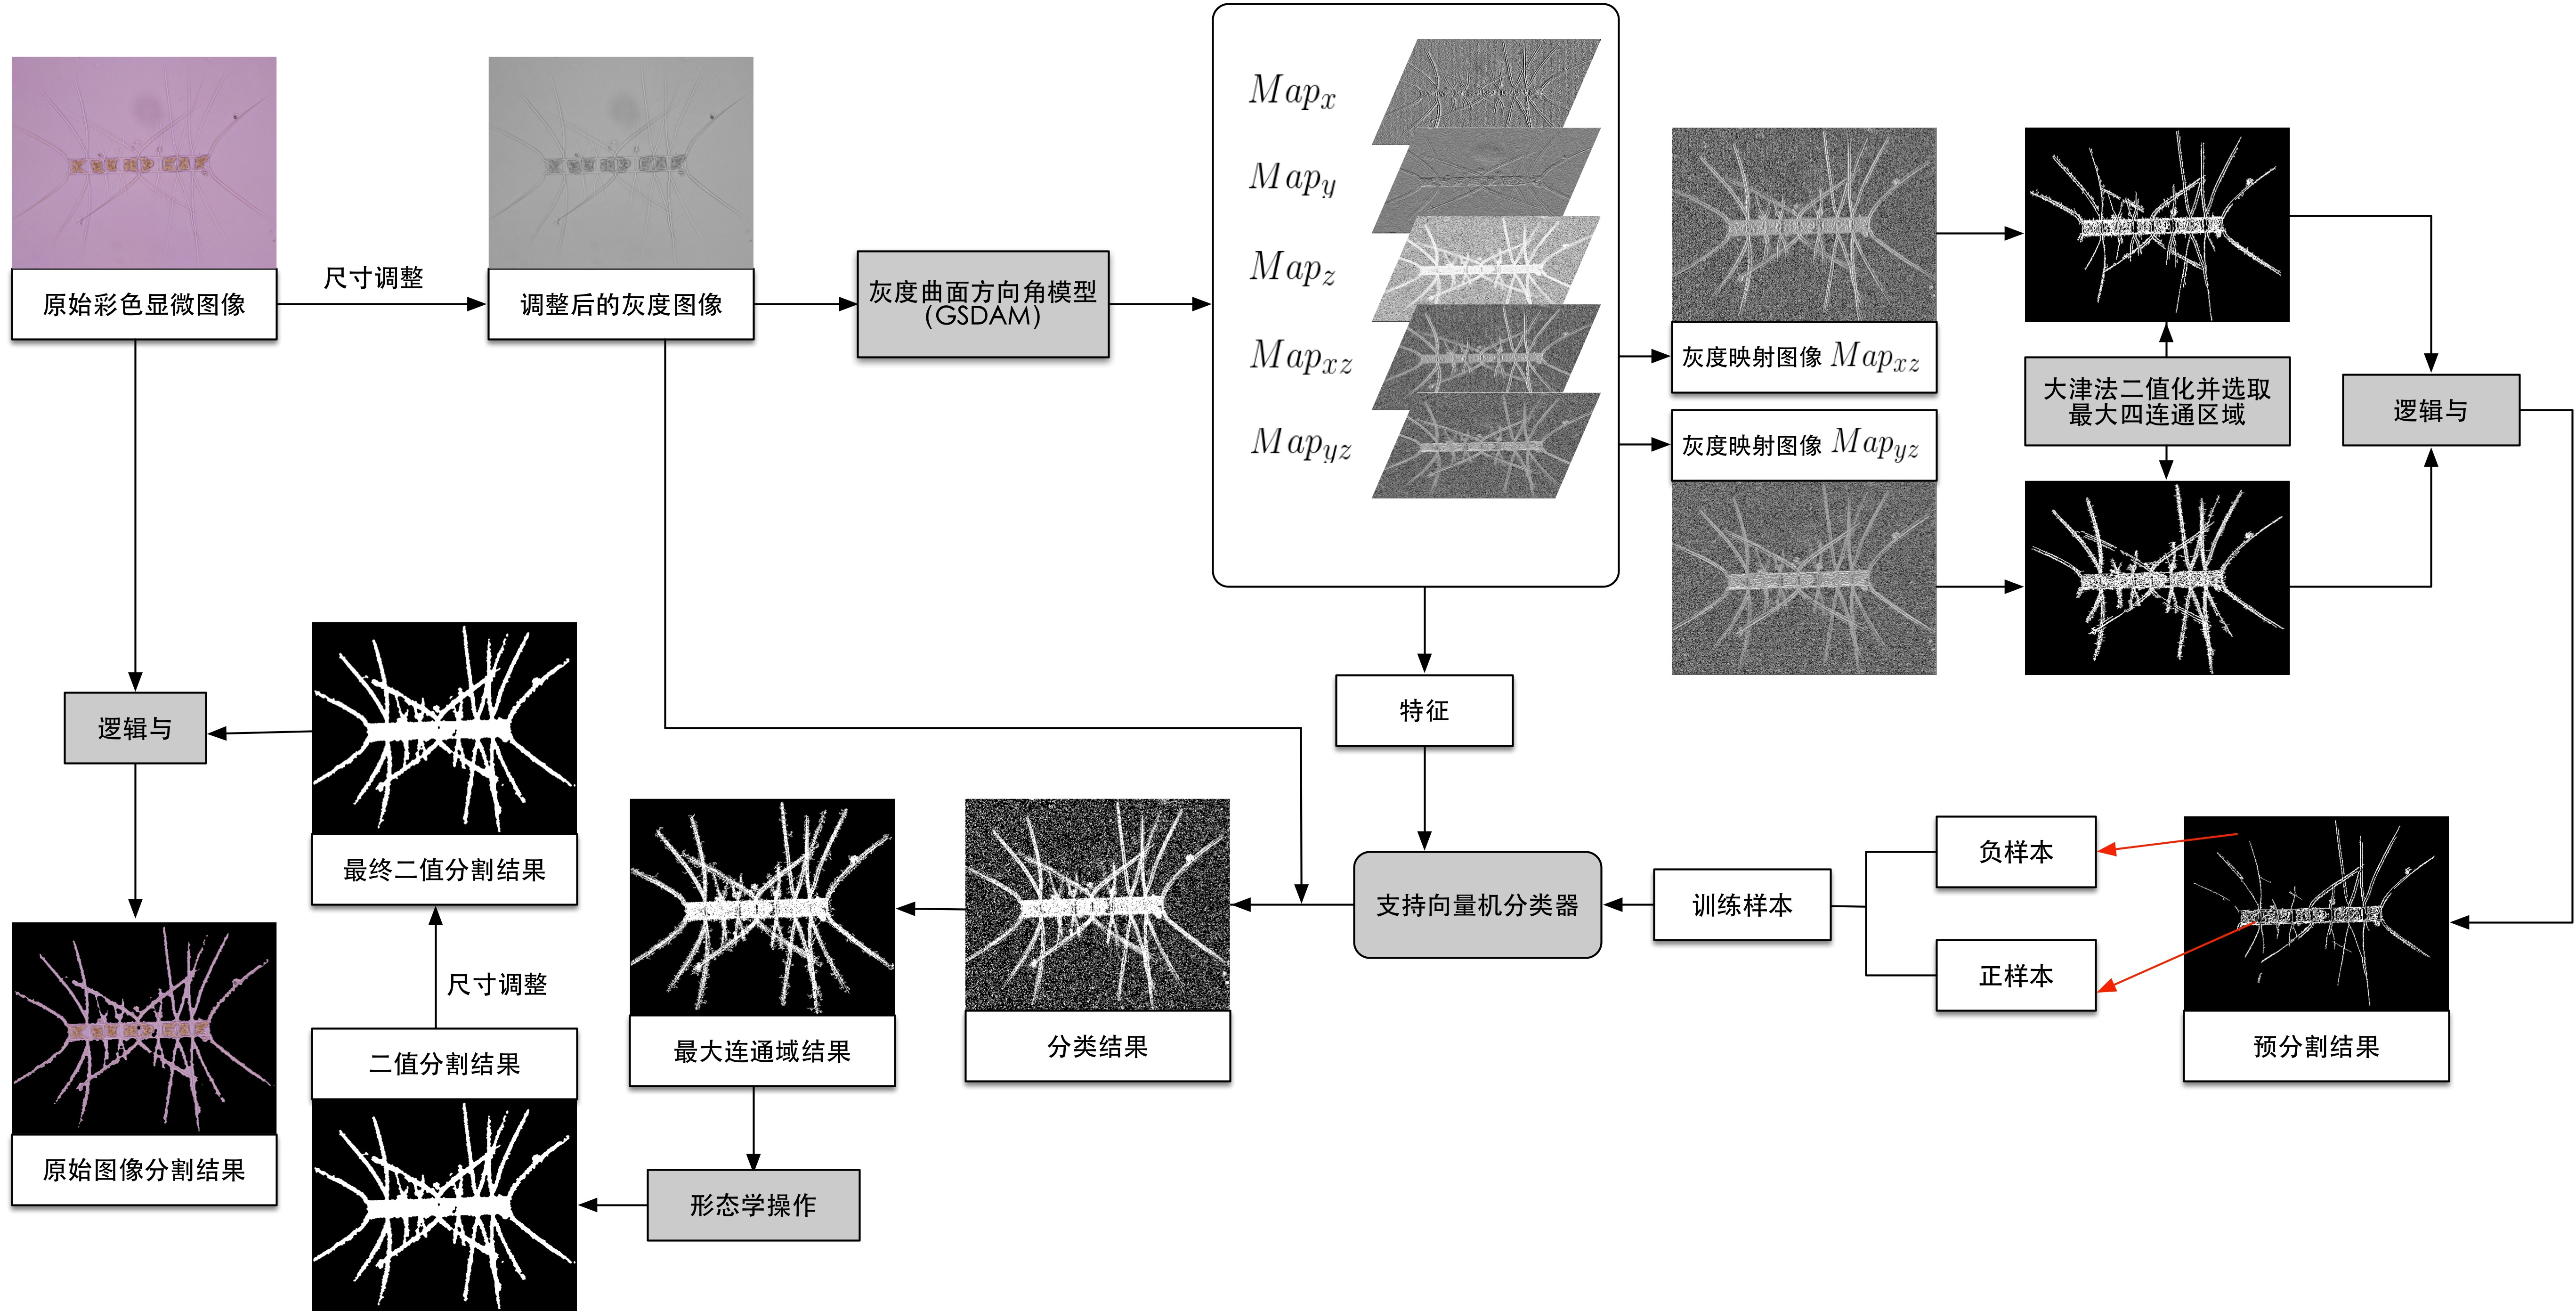
\includegraphics[width=0.9\linewidth]{flowchart.jpg}
  \caption{基于灰度曲面方向角模型和支持向量机的角毛藻显微图像分割算法流程图}
    \label{flowchart}
 \end{figure}

本文的内容安排如下:

第一章为绪论,主要介绍了藻类图像分割的国内外研究现状、课题背景与研究意义和本文的主要工作安排。

第二章为角毛藻显微图像的特征提取,主要根据角毛藻独特的生物形态学特征使用灰度曲面方向角模型(Grayscale Surface Direction Angle Model)来提取角毛藻的特征,使用该模型提取的特征含有大量的角毛藻角毛信息。

第三章为连通区域的预分割,主要运用大津法(Otsu)并选取最大连通域对图像进行预分割来生成后续支持向量机训练过程需要的训练样本。

第四章为支持向量机(Support Vector Machines)分类与后续处理,本文通过将分割问题转化为像素分类问题的形式,主要使用支持向量机来对角毛藻显微图像中的每个像素进行分类,最终完成目标(角毛藻)和背景(图像中除了角毛藻之外的其余部分)的二分类问题,最后通过一些简单的后续处理操作得到最终的分割结果。

第五章是总结和展望,分析总结了本文的工作并对今后的研究工作进行展望。



%%% Local Variables: 
%%% mode: latex
%%% TeX-master: t
%%% End: 

\chapter{角毛藻显微图像特征提取}
\label{cha2}
角毛藻细胞壁表面结构细微并且分布有以不同方式生长的角毛。由于角毛藻的特征主要集中在角毛上,因此在分割角毛藻显微图像过程中,能否将脚毛准确的提取出来起着决定性作用。

图\ref{jiaomaozao}所示为三种常见的角毛藻显微图像:
\begin{figure}[h]
  \centering
  \begin{subfigure}{3cm}
    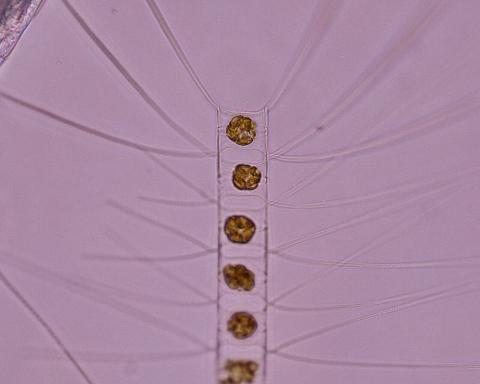
\includegraphics[height=3.5cm]{jiaomaozao1.jpg}
  \end{subfigure}
  \hspace{4em}
  \begin{subfigure}{0.2\textwidth}
    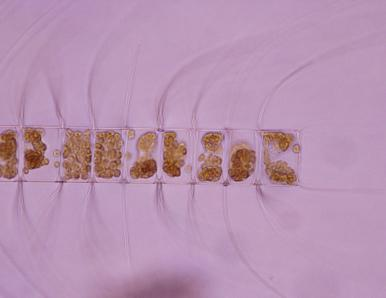
\includegraphics[height=3.5cm]{jiaomaozao2.jpg}
  \end{subfigure}
  \hspace{4em}
  \begin{subfigure}{0.25\textwidth}
    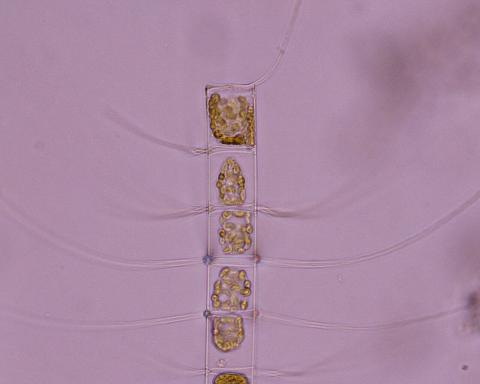
\includegraphics[height=3.5cm]{jiaomaozao3.jpg}
  \end{subfigure}
  \caption{三种常见的角毛藻显微图像}
  \label{jiaomaozao}
\end{figure}

通过对图\ref{jiaomaozao}中三种图像的观察,可以发现角毛藻的显微图像具有以下三个特征:
\begin{enumerate}
\item角毛部分长而细,并且其颜色通常与背景十分相近;
\item一些角毛藻显微图像中背景部分含有大量噪声且不易去除;
\item 图像中角毛藻的边缘部分,特别是角毛的边缘部分模糊不清呈条状分布。
\end{enumerate}

为了有效的提取尽可能多的角毛信息,本章运用了一种提取角毛藻角毛特征的基于灰度曲面方向角模型的方法。
\section{灰度曲面方向角模型}
 灰度曲面方向角模型(Grayscale Surface Direction Angle Model)是由中国海洋大学郑海永\cite{zheng2014automatic}等于2014年提出的,基于该模型的从角毛藻显微图像中分割出角毛的算法能够比传统基于边缘或基于区域的分割方法得到更好的分割结果。

一副给定的图像上的每一个像素点都可以确定一个对应的灰度曲面。由于某一点的法向量在大小为的曲面中难以确定,因此采用近似处理来确定法向量。给定一点,首先分别求出该点及其三个相邻像素点构成的四个平面的法向量,再对四个法向量求取平均值来近似表示该点的法向量。灰度曲面方向角模型的具体算法过程如下:
\begin{figure}[ht!]
   \centering
  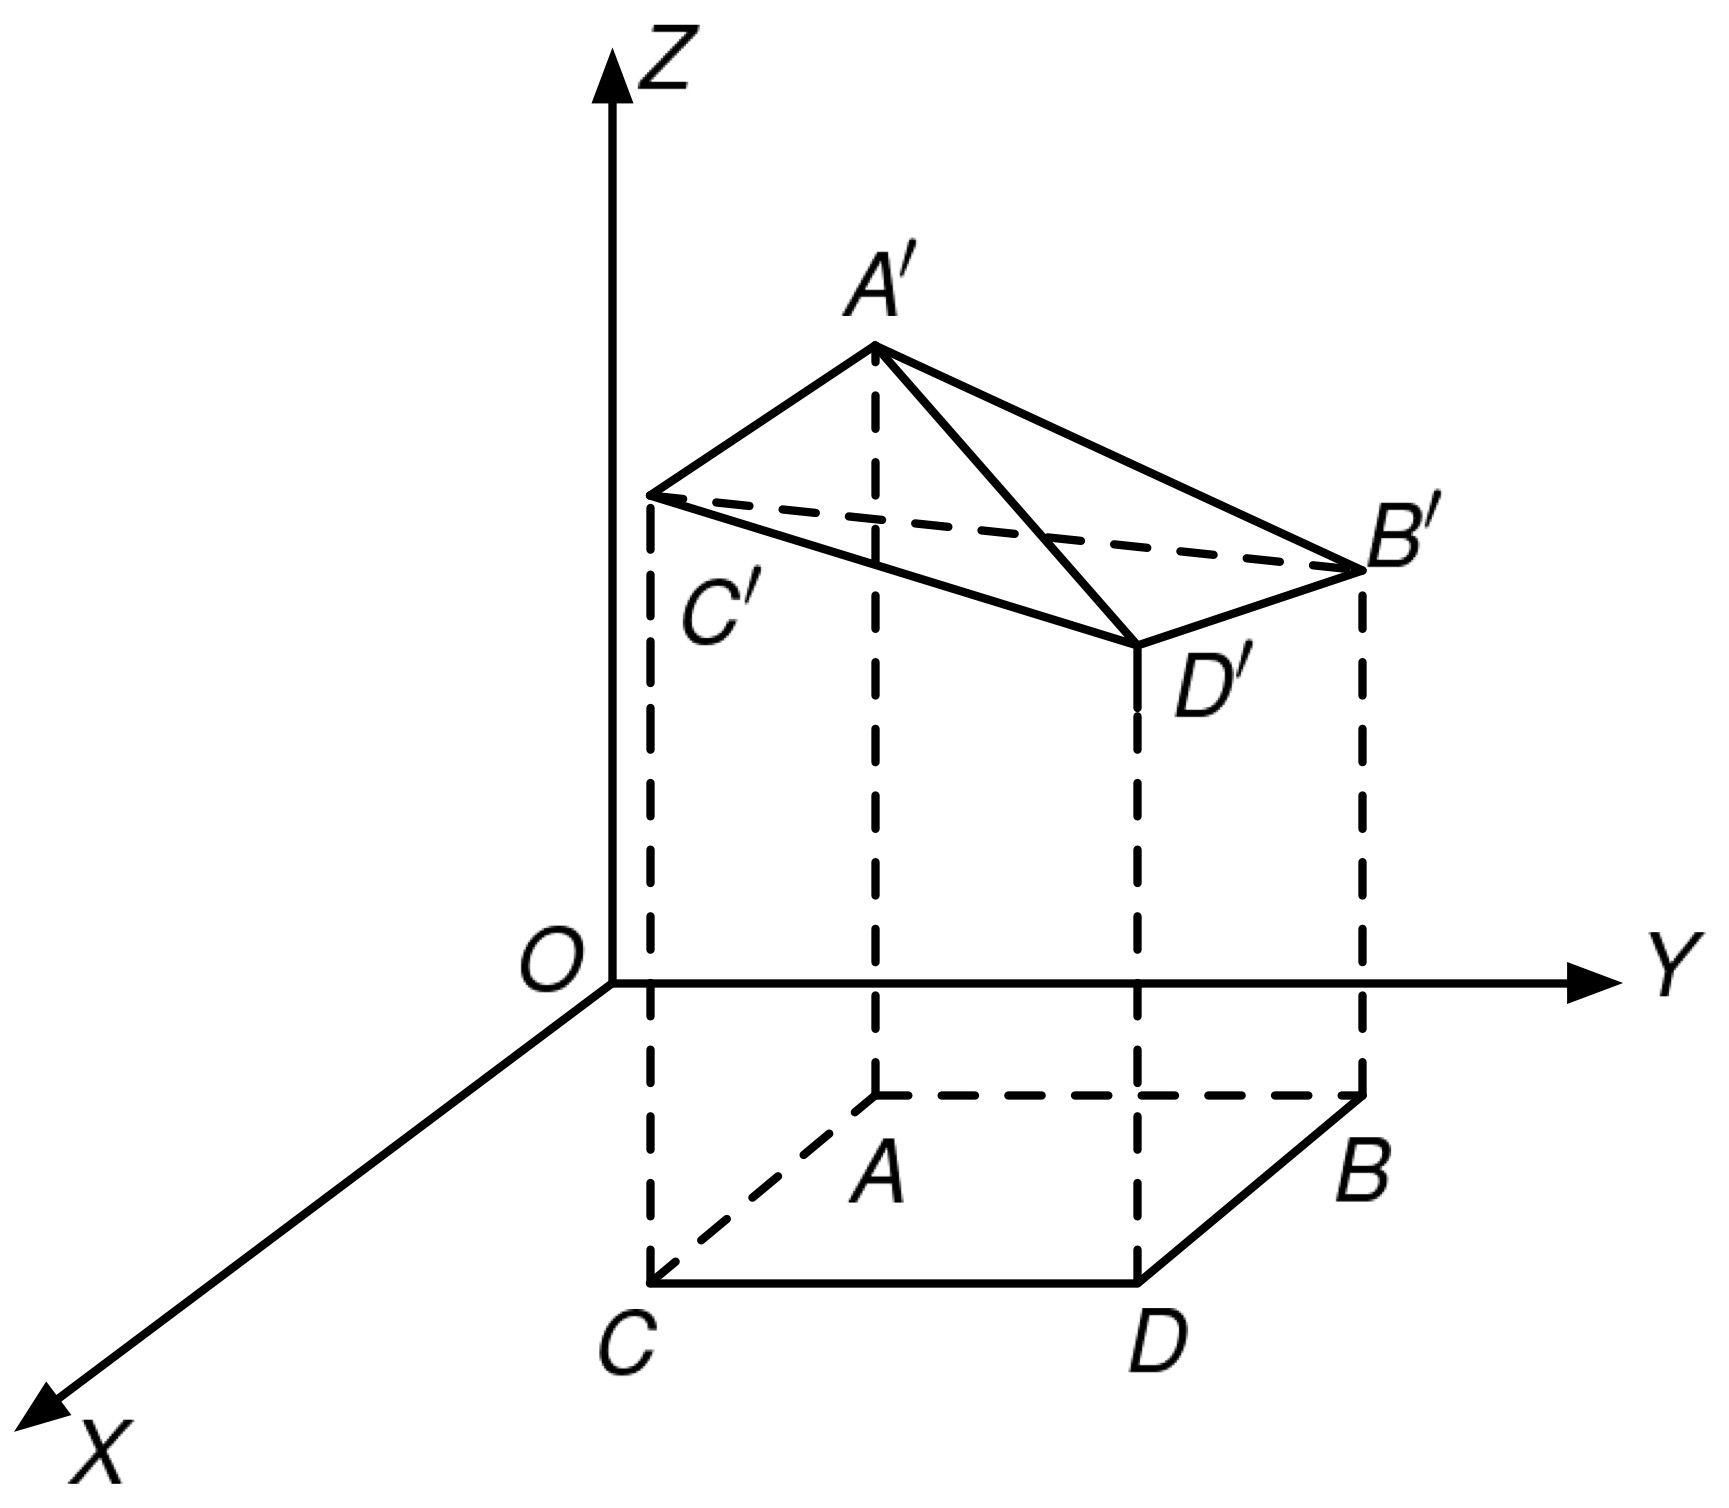
\includegraphics[width=0.8\linewidth]{figure.jpg}
  \caption{灰度曲面方向角模型的建立}
   \label{GSDAM}
 \end{figure}
 
如图\ref{GSDAM},对整副图片建立空间直角坐标系坐标系,其中$(X,Y)$是像素的空间位置,$Z$是该像素对应的灰度值。对于一个给定的像素点$A$可以确定其位置和灰度值,像素点的三个相邻的像素点分别为$B$、$C$和$D$。在空间直角坐标系中,$A$、$B$、$C$、$D$四个点分别对应$A'$、$B'$、$C'$、$D'$并且这四个点可以形成四个互不重叠的三角形面$A'B'C'$、$A'C'D'$、$A'B'D'$和$B'C'D'$。

以平面$A'B'C'$为例,平面$A'B'C'$的法向量$\overrightarrow{f_{A'B'C'}}$可以通过$\overrightarrow{f_{A'B'C'}}=\overrightarrow{A'C'}\times\overrightarrow{A'B'}$来计算,其中向量$\overrightarrow{A'C'}=(1,0,I(i+1,j)-I(i,j))$ ,向量$\overrightarrow{A'B'}=(0,1,I(i,j+1)-I(i,j))$。使用同样的方法分别计算出其余平面的法向量$\overrightarrow{f_{A'C'D'}}$、$\overrightarrow{f_{A'B'D'}}$、$\overrightarrow{f_{B'C'D'}}$,则可以利用四个三角形面的法向量近似得到的法向量:
\begin{equation}
\overrightarrow{f_{A'}}=(\overrightarrow{f_{A'B'C'}}+\overrightarrow{f_{A'C'D'}}+\overrightarrow{f_{A'B'D'}}+\overrightarrow{f_{B'C'D'}})/4
\end{equation}
通过$A'$的法向量$\overrightarrow{f_{A'}}$,可以计算出该法向量与空间直角坐标系三个坐标轴之间的夹角如下:
\begin{equation}
\begin{split}
\theta_{x}(i,j)=360\times \cos ^{-1}(f_{x}/|\overrightarrow {f_{A'}}| )/2\pi\\
\theta_{y}(i,j)=360\times \cos ^{-1}(f_{y}/|\overrightarrow {f_{A'}}| )/2\pi\\
\theta_{z}(i,j)=360\times \cos ^{-1}(f_{z}/|\overrightarrow {f_{A'}}| )/2\pi
\end{split}
\end{equation}
其中$f_{x}$、$f_{y}$、$f_{z}$分别是$\overrightarrow{f_{A'}}$在轴$X$、$Y$、$Z$的坐标值,$|\overrightarrow {f_{A'}}|$是$\overrightarrow{f_{A'}}$的模。
依次对范围在$[\min(\theta),\max(\theta)]$的三个夹角$\theta_{x}$、$\theta_{y}$、$\theta_{z}$进行灰度映射,映射后其范围在$[0,255]$之间:
\begin{equation}
\begin{split}
Map_{x}(i,j)=255\times\frac{\theta_{x}(i,j)-\min(\theta_{x})}{\max(\theta_{x})-\min(\theta_{x})}\\
Map_{y}(i,j)=255\times\frac{\theta_{y}(i,j)-\min(\theta_{y})}{\max(\theta_{y})-\min(\theta_{y})}\\
Map_{z}(i,j)=255\times\frac{\theta_{z}(i,j)-\min(\theta_{z})}{\max(\theta_{z})-\min(\theta_{z})}
\end{split}
\end{equation}
此外还可以得到$xz$平面和$yz$平面的灰度映射:
\begin{equation}
\begin{split}
Map_{xz}(i,j)=\sqrt{Map_{x}(i,j)^{2}+Map_{z}(i,j)^{2}}\\
Map_{yz}(i,j)=\sqrt{Map_{y}(i,j)^{2}+Map_{z}(i,j)^{2}}
\end{split}
\end{equation}
利用同样的方法来处理图像中的所有像素可以得到五张灰度图像$Map_{x}$、$Map_{y}$、$Map_{z}$、$Map_{xz}$、$Map_{yz}$,对于图像右侧和下侧边缘部分的像素,可以采取重复边缘灰度值的方式来扩展图像边缘。
\section{实验结果}
\subsection{实验前的预处理操作}
由于选取的数据集中原始彩色角毛藻图像的尺寸非常大,在后续SVM训练和预测过程中运算复杂度很高、耗时较长,因此为了降低运算复杂度并减少运算时间,将角毛藻显微图像调整至原来尺寸的0.15倍。

此外,考虑到显微图像的颜色会因成像设备和滤波器的不同而产生差异,在实验开始前需要将原始调整后的RGB显微图像转化成灰度图像。此时,每一幅灰度图像都可以视为一个空间直角坐标系。
\begin{figure}[ht!]
\centering
\begin{minipage}[b]{0.45\linewidth} 
      \centering 
      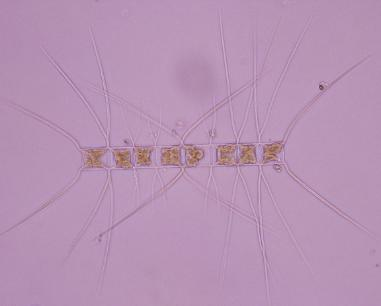
\includegraphics[width=0.9\linewidth]{resize.jpg}
        \centerline{(a) 原始显微图像}\medskip
\end{minipage}
  \begin{minipage}[b]{0.45\linewidth}
    \centering
    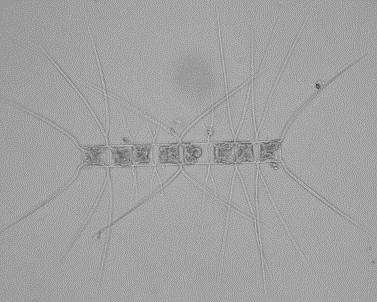
\includegraphics[width=0.9\linewidth]{resize_gray.jpg}
      \centerline{(b) 调整后灰度图像}\medskip
  \end{minipage}
 \caption{实验前的预处理操作}
\end{figure}

\subsection{角毛藻显微图像特征提取结果}
对每一幅原始灰度图像中的所有像素使用灰度平面方向角模型方法进行处理操作可以得到五张含有角毛藻目标细胞和角毛特征信息的灰度映射图像,这五副灰度图可以用作后续支持向量机分类器的输入特征。

如图\ref{GSDAMresults}所示为并基角毛藻显微图像的特征提取结果:

\begin{figure}[ht!]
\centering
    \begin{minipage}[b]{0.45\linewidth}
    \centering
    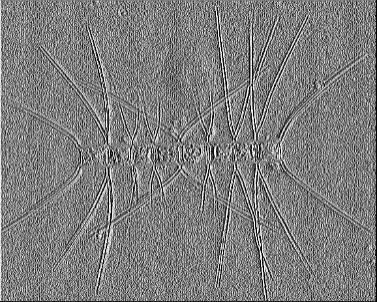
\includegraphics[width=0.9\linewidth]{mapx.jpg}
      \centerline{(a) x方向灰度映射图}\medskip
  \end{minipage}
  \begin{minipage}[b]{0.45\linewidth}
    \centering
    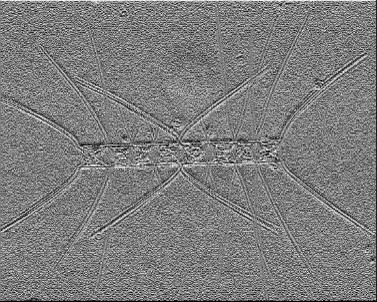
\includegraphics[width=0.9\linewidth]{mapy.jpg}
      \centerline{(b) y方向灰度映射图}\medskip
  \end{minipage}
   \begin{minipage}[b]{0.45\linewidth}
    \centering
    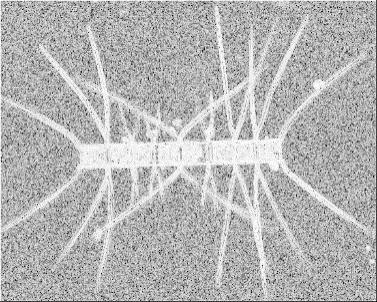
\includegraphics[width=0.9\linewidth]{mapz.jpg}
      \centerline{(c) z方向灰度映射图}\medskip
  \end{minipage}
  \begin{minipage}[b]{0.45\linewidth}
    \centering
    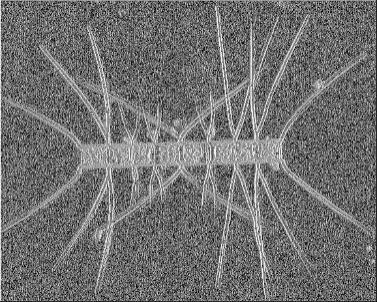
\includegraphics[width=0.9\linewidth]{mapxz.jpg}
      \centerline{(d) xz方向灰度映射图}\medskip
  \end{minipage}
   \begin{minipage}[b]{0.45\linewidth}
    \centering
    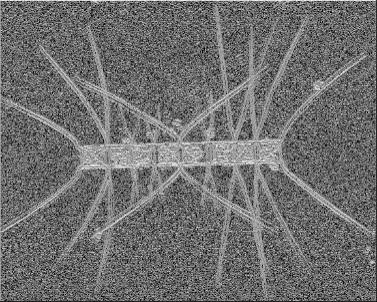
\includegraphics[width=0.9\linewidth]{mapyz.jpg}
      \centerline{(e) yz方向灰度映射图}\medskip
  \end{minipage}
 \caption{角毛藻显微图像的特征提取结果}
  \label{GSDAMresults}
\end{figure}


\section{本章小结}
本章针对角毛藻独特的生物形态学特征,使用灰度曲面方向角模型对角毛藻显微图像进行特征提取。

首先介绍了灰度曲面方向角模型的基本原理,然后通过实验验证了采用灰度平面方向角模型的特征提取方法能够较为准确的提取出角毛等特征信息,有助于后续操作中利用连通区域预分割产生支持向量机的训练样本,并且可以作为支持向量机的输入特征。


%\usepackage{algorithm}
%\usepackage{algorithmic}

\chapter{连通区域的预分割}
由上述章节可知,利用灰度曲面方向角模型来处理原始角毛藻显微灰度图像可以得到五张灰度特征图。其中$Map_{xz}$和$Map_{yz}$的灰度映射值较大,因此保留有大量的角毛和细胞边缘特征信息,可以更好的分割具有噪声的低对比度角毛藻显微图像的角毛。因此在这一章节中,将主要利用$Map_{xz}$和$Map_{yz}$来进行预分割的一系列操作,通过这些操作产生的结果将被用来作为支持向量机的训练样本。本章所使用的方法主要分为大津法和最大连通域的选取。
\section{大津法}
大津法(又称:最大类间方差法,OTSU)是由日本学者大津展之\cite{otsu1975threshold}于1979年提出的,是一种自适应的确定阈值来实现图像二值化的高效方法。大津法通过图像灰度特性将图像分为目标和背景两部分,通过选取目标和背景间的最大类间方差和最小类内方差来确定最佳阈值。

假设$t$为将整副图像灰度级划分为两类的阈值:$C_{0}=(0,1,...,t)$和$C_{1}=(t+1,t+2,...,L-1)$。$C_{0}$和$C_{0}$的概率分别表示为:
\begin{equation}
\omega_{0}=\sum_{i=0}^{t}P_{i}=\omega(t)
\end{equation}

\begin{equation}
\omega_{1}=\sum_{i=t+1}^{L-1}P_{i}=1-\omega(t)
\end{equation}

均值分别表示为:
\begin{equation}
\mu_{0}=\sum_{i=0}^{t}iP_{i}/\omega_{0}=\mu(t)/\omega(t)
\end{equation}

\begin{equation}
\mu_{1}=\sum_{i=t+1}^{L-1}iP_{i}/\omega_{1}=\frac{\mu_{T}(t)-\mu(t)}{1-\omega(t)}
\end{equation}

其中,$\mu(t)=\sum_{i=0}^{t}iP_{i}$,$\mu_{T}(t)=\sum_{i=0}^{L-1}iP_{i}$。对于任意的t值,都满足:$\omega_{0}\mu_{0}+\omega_{1}\mu_{1}=\mu_{T}$且$\omega_{0}+\omega_{1}=1$。

$C_{0}$和$C_{0}$的方差分别表示为:
\begin{equation}
\sigma_{0}^{2}=\sum_{i=0}^{t}(i-\mu_{0})^2P_{i}/\omega_{0}
\end{equation}

\begin{equation}
\sigma_{1}^{2}=\sum_{i=t+1}^{L-1}(i-\mu_{1})^2P_{i}/\omega_{1}
\end{equation}
定义类内方差为:
\begin{equation}
\sigma_{w}^{2}=\omega_{0}\sigma_{0}^{2}+\omega_{1}\sigma_{1}^2
\end{equation}
类间方差为:
\begin{equation}
\sigma_{B}^{2}=\omega_{0}(\mu_{0}-\mu_{T})^{2}+\omega_{1}(\mu_{1}-\mu_{T})^{2}=\omega_{0}\omega_{1}(\mu_{1}-\mu_{0})^{2}
\end{equation}
总体方差为:
\begin{equation}
\sigma_{T}^{2}=\sigma_{w}^{2}+\sigma_{B}^2
\end{equation}
引入判别准则:
\begin{equation}
\eta(t)=\frac{\sigma_{B}^{2}}{\sigma_{T}^{2}}
\end{equation}
将阈值$t$从图像最小灰度级到最大灰度级依次设置,并计算相应的值,比较所有$\eta(t)$值大小,找出$\eta(t)$取最大值时的$t^{*}值$:
\begin{equation}
t^{*}=\argmax_{0\le t\le L-1}\eta(t)
\end{equation}
目标和背景之间的类间方差越大说明目标和背景之间的灰度差别越大,与之相反,二者间的类间方差越小说明目标和背景之间的灰度差别越小即灰度分布越均匀,若出现错分现象即部分背景被错误地分为目标区域或部分目标被错误地分为背景区域都会使这两部分的差别变小,所以使错分几率达到最小就意味着需要获取最大的类间方差。


\section{实验结果}
首先采用大津法将灰度映射图$Map_{xz}$和$Map_{yz}$转化成二值图像,转化后的两幅二值图像包含两类像素即目标像素和背景像素。

然后利用MATLAB函数bwlabel标记两幅二值图像的四连通领域,被标记为0的像素为背景,其余标记如被标记为1的像素组成第一区域,被标记为2的像素组成第二区域。保留二值图像中的最大连通区域即像素值最多的区域并且移除二值图像中的其他区域,可以得到两幅保留较多角毛藻特征信息的二值图像。

因为原始角毛藻灰度图像中的噪声没有方向性和规律性,并且比较杂乱,不能同时在两幅得到的二值图像上得到高的灰度值,所以需要对两幅得到的二值图像使用逻辑“与”(AND)操作来尽量减少较为显著的噪声从而更加突出角毛藻的脚毛和细胞边缘信息。最终可以得到一个精确但是仍然缺少某些特征信息的不完整的角毛藻二值预分割结果。所得的预分割结果将会被用来作为支持向量机训练过程中的训练样本。

如图\ref{trainingsampleresult}所示为实验结果:
\begin{figure}
\centering
    \begin{minipage}[b]{0.45\linewidth}
    \centering
    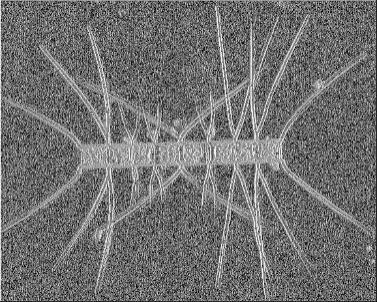
\includegraphics[width=0.9\linewidth]{mapxz.jpg}
      \centerline{(a) xz方向灰度映射图}\medskip
  \end{minipage}
  \begin{minipage}[b]{0.45\linewidth}
    \centering
    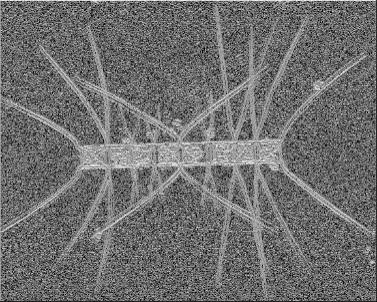
\includegraphics[width=0.9\linewidth]{mapyz.jpg}
      \centerline{(b) yz方向灰度映射图}\medskip
  \end{minipage}
   \begin{minipage}[b]{0.45\linewidth}
    \centering
    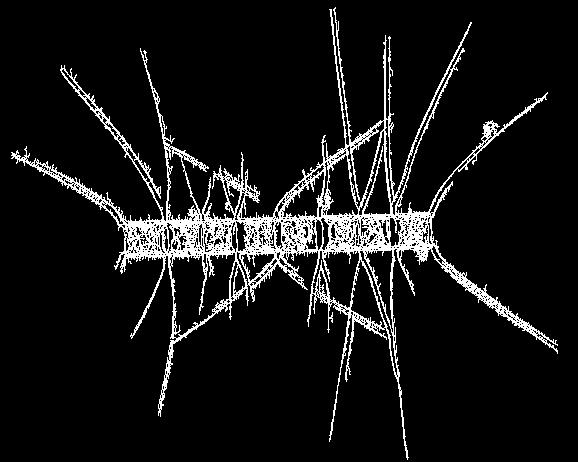
\includegraphics[width=0.9\linewidth]{xz.jpg}
      \centerline{(c) xz方向对应处理结果}\medskip
  \end{minipage}
  \begin{minipage}[b]{0.45\linewidth}
    \centering
    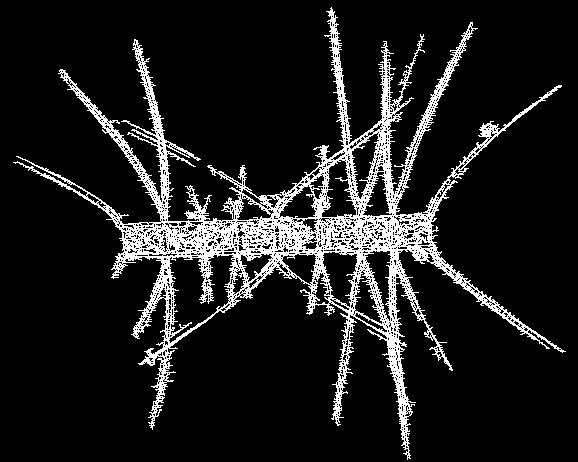
\includegraphics[width=0.9\linewidth]{yz.jpg}
      \centerline{(d) yz方向对应处理结果}\medskip
  \end{minipage}
   \begin{minipage}[b]{0.45\linewidth}
    \centering
    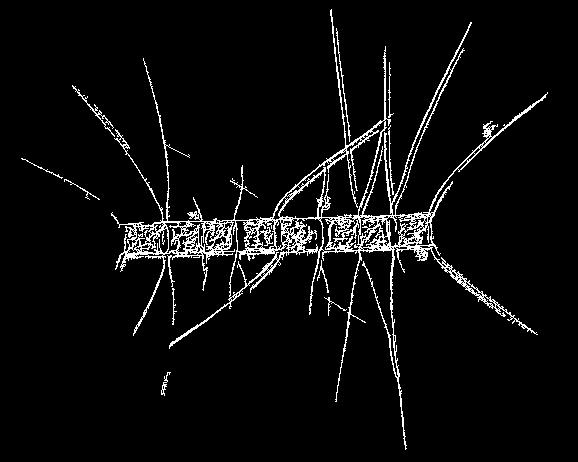
\includegraphics[width=0.9\linewidth]{traingingsample.jpg}
      \centerline{(e) 最终预分割结果}\medskip
  \end{minipage}
 \caption{大津法二值化与选取最大连通区域的预分割结果}
  \label{trainingsampleresult}
\end{figure}

\section{本章小结}
本章主要使用大津法和选取最大连通域来获取角毛藻显微图像的预分割结果。首先选择xz和yz方向的灰度映射图进行大津法二值化,然后使用最大连通域填充,最后通过逻辑“与”操作获取最终的预分割结果,得到的预分割结果将作为后续支持向量机分类训练过程的训练样本。

%%% Local Variables: 
%%% mode: latex
%%% TeX-master: t
%%% End: 

\chapter{支持向量机分类与后续处理}
 图像分割问题本质上是一个分类问题,图像中的所有像素都被分成两类或者更多类。每一类像素都有共有的特征,分类过程通过这些特征将每一类区分出来。传统的分类方法有监督方法和非监督方法,比如说支持向量机\cite{cortes1995support},K-means聚类方法\cite{macqueen1967some}和朴素贝叶斯分类器\cite{rish2001empirical}等。本文采用支持向量机来对角毛藻显微图像中的所有像素进行分类,待处理图像中的像素被分为两类:目标部分(角毛藻)和背景部分。由于经过分类后的图像并没有完全把目标分离出来,因此还需要通过后续处理来生成最终的分割结果。

\section{支持向量机}
支持向量机(Support Vector Machine,SVM)理论,是Corinna Cortes和Vapnik\cite{cortes1995support}等于1995年首先提出的,因为它在解决非线性、小样本及高维模式识别中表现出许多特有的优势,并且能推广应用到其他机器学习问题中,所以一直被认为是效果最好的可用的分类算法之一。在机器学习领域中,受到越来越多的广泛关注。

传统的学习方法一般是通过最小化经验风险(Empirical Risk Minimization,ERM)来实现的。但是当只有有限个训练样本时,经验风险最小化原则一般是不合理的,并且ERM算法在实际应用中会遇到不适定等问题。

支持向量机是通过寻求结构化风险最小来提高学习机的泛化能力,最小化经验风险和置信范围以达到在样本量较少情况下仍能获得较好统计规律的目的。其基本思想是:当样本集是线性时,两类样本通过寻找最优分类超平面来区分;当样本集是非线性时,需要将低维空间映射到高维空间来寻找最优分类超平面。支持向量机通过使用具有某些特殊性质的核函数将特征空间中的内积运算转换为在低位空间里的非线性运算,避免了高维空间的计算问题。
    
\subsection{实际风险、经验风险与结构风险}
\subsubsection{实际风险}
假设学习机器广义参数为$\omega$,那么对于输入量和输出量分别为$x$和$f(x,\omega)$的学习机器,其预测的实际风险为:
\begin{equation}
R(\alpha)=\int L(y,f(x,\omega))dF(x,y)
\end{equation}
$F(x,y)$为变量$x$和$y$之间的联合分布,$L(y,f(x,\omega))$则为损失函数,即预测输出$f(x,\omega)$对实际输出$y$预测产生的损失。

\subsubsection{经验风险}
在实际应用中,联合分布$F(x,y)$是不可能得到的,经验风险最小化原则一般会通过样本来对经验风险定义:
\begin{equation}
R_{emp}(\omega)=\frac{1}{n}\sum_{i=1}^{n}L(y_{i}.f(x_{i},\omega))
\end{equation}

优化机器学习就是要找到一个最优广义参数$\alpha$并最小化$R(\alpha)$,最小化经验风险实质上就是使经验风险逐渐趋近于实际风险的过程。

此外由于经验风险是基于大数定律得到的,$R_{emp}$只有样本趋于无穷时才能在概率意义上趋于$R(\alpha)$。因此在样本数有限的情况下是否能取得良好的结果仍然缺乏理论支持。

\subsubsection{结构风险}
对于所有预测函数来说,$R(\alpha)$与$R_{emp}$间以大于等于$1-\eta$的概率满足以下关系:
\begin{equation}\label{gongshi}
R(\alpha)\le R_{emp}(\omega)+\sqrt{\frac{(h(\ln(\frac{2n}{h})+1)-\ln(\frac{\eta}{4})}{n}}
\end{equation}
其中,$n$表示样本数,$h$表示函数集的VC维(Vapnik-Chervonenkis Dimension),由式\ref{gongshi}可知,置信范围和经验风险两部分共同组成了实际风险。在实际机器学习过程中,最小化经验风险同时尽最大可能减少置信范围,并且按照VC维的大小,综合衡量$R_{emp}$和函数子集间的置信范围来获取$R(\alpha)$的最小值的思想就是结构风险最小化(Structural Risk Minimization),即SRM准则。

\subsection{线性情况与非线性情况} 
\subsubsection{线性情况} 

首先考虑一个两类的分类问题,数据点$x$是一个$n$维向量,类别用$y$表示,取值可以是$1$或$-1$。线性分类器就是要从$n$维的数据空间中找出一个超平面来将整个数据空间分为两类,其方程可以表示为:
\begin{equation}
w^{T}x+b=0
\end{equation}
一个超平面在二维空间中就是一条直线,令分类函数$f(x)=w^{T}x+b$,当$f(x)=0$时,$x$是位于超平面上的点。对于所有满足$f(x)<0$的点,其对应的$y=-1$;而满足$f(x)>0$则对应$y=1$的数据点。$\vert f(x)\vert$越大分类越容易,当$\vert f(x)\vert=0$或$\vert f(x)\vert$值很小时,通常情况下很难处理。因为出现比较细微的变动(比如超平面转动了一个很小的角度时)很可能会导致分类结果的变化。直观几何意义上来说,越远离超平面的点越容易分类,而接近超平面的点往往很难分类。
\begin{figure}[ht!]
   \centering
  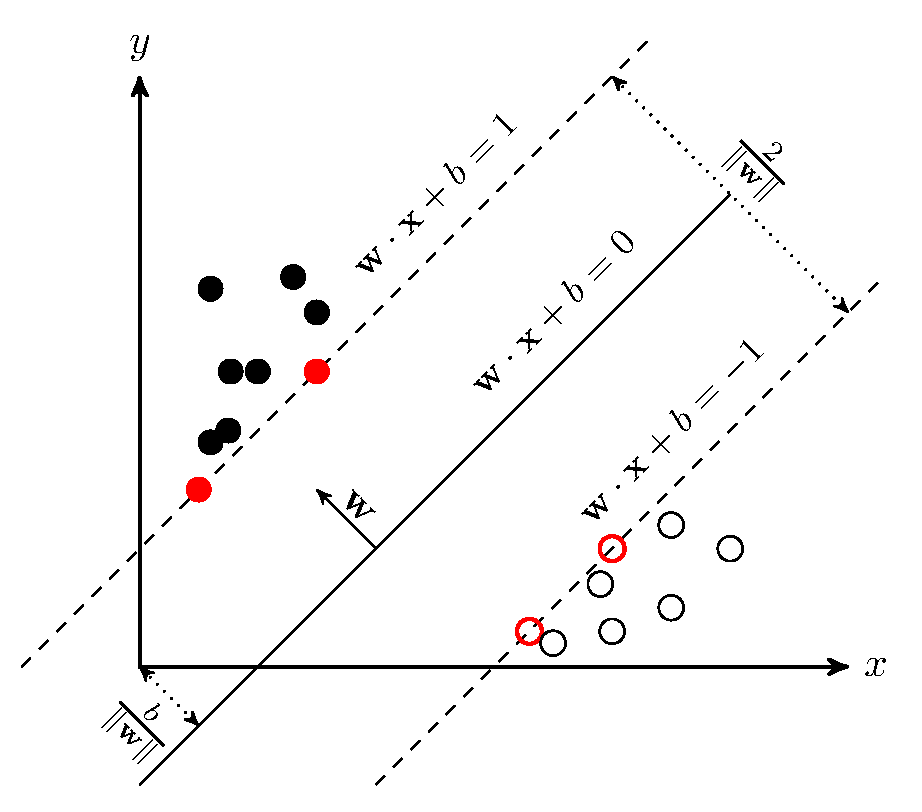
\includegraphics[width=0.9\linewidth]{svm.png}
  \caption{最优超平面}
    \label{}
 \end{figure}


假设一个数据点$x$投影到超平面上为$x_{0}$,$w$为垂直于超平面的矢量,则$x$到超平面的几何间隔为:
\begin{equation}
\hat{\gamma}=y\gamma=\frac{\hat{\gamma}}{\Vert{w}\Vert}
\end{equation}
其中$\hat{\gamma}$为函数间隔,且$\hat{\gamma}=y(w^{T}x+b)=yf(x)$,当对数据点进行分类时,集合间隔越大,分类置信就越高。因此为了使得分类的置信高,希望选择的超平面能够最大化几何间隔,定义目标函数为:
\begin{equation}
\max \hat{\gamma}
\end{equation}
当然还需要满足一些条件,根据间隔的定义,有:
\begin{equation}
y_{i}(w^{T}x+b)=\hat{\gamma_{i}}\ge\hat{\gamma},i=1,...,n
\end{equation}
为了优化和方便推导,令$\hat{\gamma}=1$,则上述目标函数变为:
\begin{equation}
\max\frac{1}{\Vert{w}\Vert},s.t.,y_{i}(w^{T}x+b)\ge1,i=1,...,n
\end{equation}
上述问题等价于:
\begin{equation}
\max\frac{1}{2}\Vert{w}\Vert^{2},s.t.,y_{i}(w^{T}x+b)\ge1,i=1,...,n
\end{equation}
使用拉格朗日优化法改造上式,即在满足$\sum_{i=1}^{n}y_{i}\alpha_{i}=0$
和$\alpha_{i}\ge0,i=1,...,n$的约束条件下,求解下式:
\begin{equation}
Q(\alpha)=\max \sum_{i=1}^{n}\alpha_{i}-\frac{1}{2}\sum_{i,j=1}^{n}\alpha_{i}\alpha_{i}y_{i}y_{j}(x_{i}\bullet x_{j})
\end{equation}
$\alpha_{i}$是每一个样本对应的拉格朗日乘子,上式有唯一解,只有当对应样本是支持向量时,$\alpha_{i}$不为零。则可以得到最优分类函数为:
\begin{equation}
g(x)=\textrm{sgn}\{(w\bullet x)+b\}=\textrm{sgn}\Big \{\sum_{i=1}^{n}\alpha_{i}^{*}y_{i}(x_{i}\bullet x)+b^{*}\Big \}
\end{equation}
只需要对支持向量求和并计算任意一对支持向量的中指或代入到任意一个支持向量都可以求出分类阈值$b^{*}$。

\subsubsection{非线性情况} 
当需要分类的训练集是非线性时,需要通过映射$\phi(\cdot)$将训练集映射到高维空间上。在高维空间上,训练集是线性可分的,决策函数可以通过采用线性情况的形式来构造最优分类超平面。支持向量机允许数据点在一定程度上偏离超平面。此时,约束条件变为:
\begin{equation}
y_{i}(w^{T}x+b)\ge 1-\xi_{i},i=1,...,n
\end{equation}
$\xi_{i}$是松弛变量,表示数据点$x_{i}$允许偏离的函数间隔值。此时的目标函数为:
\begin{equation}
\min\frac{1}{2}\Vert{w}\Vert^{2}+C\sum_{i=1}^{n}\xi_{i}
\end{equation}
\begin{equation}
s.t.,y_{i}(w^{T}x_{i}+b)\ge1-\xi_{i},i=1,...,n,\xi_{i}\ge0,i=1,...,n
\end{equation}
$C$为确定的常量,用以控制确保数据点偏差最小且能够找到间隔最大超平面的权重。$\xi$为待优化变量,目标函数为:
\begin{equation}
Q(\alpha)=\max \sum_{i=1}^{n}\alpha_{i}-\frac{1}{2}\sum_{i,j=1}^{n}\alpha_{i}\alpha_{i}y_{i}y_{j}K(x_{i},x_{j})
\end{equation}

\begin{equation}
s.t.,0\le\alpha_{i}\leC,i=1,...,n,\sum_{i=1}^{n}\alpha_{i}y{i}=0
\end{equation}
对应的分类函数变为:
\begin{equation}
g(x)=\textrm{sgn}\Big \{\sum_{i=1}^{n}\alpha_{i}^{*}y_{i}K(x_{i},x)+b^{*}\Big \}
\end{equation}

其中$K(x_{i},x_{j})=\phi(x_{i})\cdot\phi(x_{j})$为核函数。

\subsection{常见的核函数} 
当处于非线性情况时,需要将训练集映射到高维空间来寻找最优分类超平面。然而点积运算量会随着空间维数的增大而增大,这会产生“维数灾难”。支持向量机需要使用核函数来克服“维数灾难”,在选取核函数时需要满足Mercer条件,即:

\begin{equation}
\iint K(x_{i},x_{j})\phi(x_{i})\phi(x_{j})dx_{i}dx_{j}>0
\end{equation}
其中$\int\phi^{2}(x)dx<\infty$且$\phi(x)$不恒为零。
在实际情况下,通常用到以下三个核函数:
\begin{enumerate}
\item多项式核函数:
\begin{equation}
K(x_{i},x_{j})=[\gamma x_{i}\bullet x_{j}+r]^{d}
\end{equation}
\item径向基核函数:
\begin{equation}
K(x_{i},x_{j})=\exp\Big\{-\frac{\Vert x-x_{i}\Vert^{2}}{\sigma^{2}}\Big\}
\end{equation}
\item Sigmoid函数:
\begin{equation}
K(x_{i},x_{j})=\tanh[\gamma x_{i}^{T}\bullet x_{j}+r]
\end{equation}
\end{enumerate}

\section{实验结果}
本文使用支持向量机来对待处理图像中的像素进行分类,支持向量机的分类过程分为训练过程和预测过程。
\begin{enumerate}
\item训练过程:

    在训练过程中,五张灰度特征映射图和预分割结果分别作为支持向量机的输入特征和训练样本。将预分割结果中的目标部分和背景部分分别视为正样本和负样本,标记为$1$和$-1$,并选取线性核函数进行训练。
\item预测过程:

    在预测过程中,输入调整后的灰度图像和它们的五个灰度特征映射图到支持向量机中进行分类。预测完毕后,所有的像素都被标记成$1$和$-1$,并且将调整后灰度图像中目标像素灰度值置为$1$,其它则置为$0$。
\end{enumerate}

支持向量机分类完成后,图像中仍然含有一定的噪声,因此需要再次进行连通域操作来选取目标部分的最大连通域。此外,还需要加入一些形态学操作来平滑边缘并填充目标,这时可以得到一个调整后的二值图像。同时,获取的结果需要再一次进行调整恢复成原始二值图像。最后,对原始二值图像和原始彩色显微图像使用逻辑“与”操作来得到最终图像分割结果。

具体实验结果如下图\ref{svm}所示。
\begin{figure}[!ht]
  \centering
  \begin{subfigure}{0.3\textwidth}
   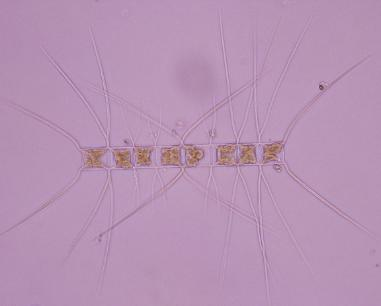
\includegraphics[height=3.6cm]{resize.jpg}
   \caption{}
  \end{subfigure}
  \begin{subfigure}{0.3\textwidth}
    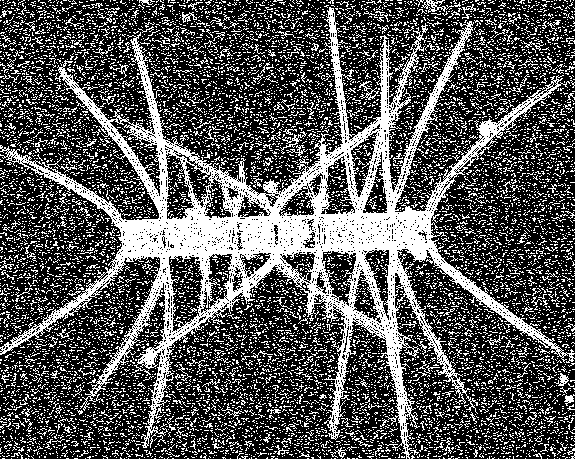
\includegraphics[height=3.6cm]{bingji1svm.png}
    \caption{}
  \end{subfigure}
  \begin{subfigure}{0.3\textwidth}
    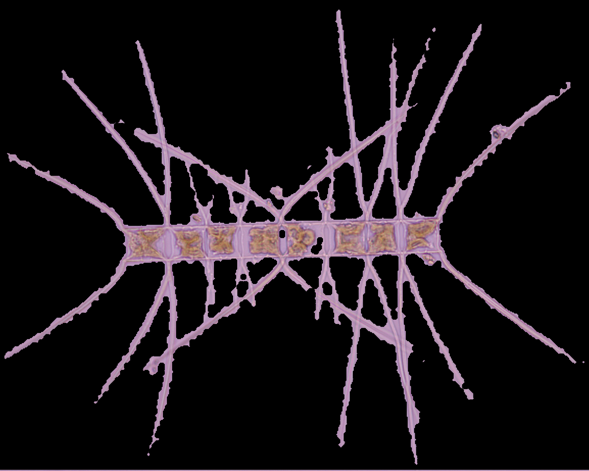
\includegraphics[height=3.6cm]{bingji1result.png}
    \caption{}
  \end{subfigure}
  \\
  \begin{subfigure}{0.3\textwidth}
    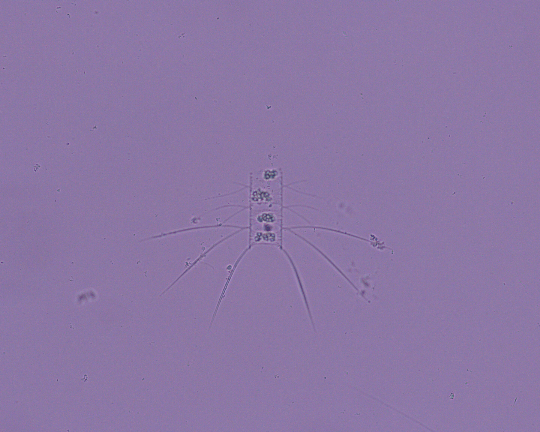
\includegraphics[height=3.6cm]{bingji2.png}
    \caption{}
  \end{subfigure}
 \begin{subfigure}{0.3\textwidth}
    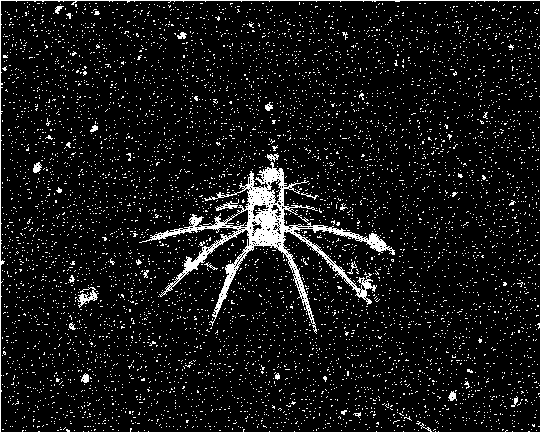
\includegraphics[height=3.6cm]{bingji2svm.png}
    \caption{}
  \end{subfigure}
 \begin{subfigure}{0.3\textwidth}
    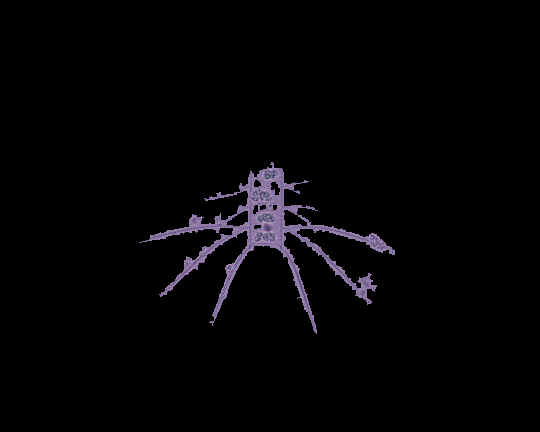
\includegraphics[height=3.6cm]{bingji2result.png}
    \caption{}
  \end{subfigure}
 \\
 \begin{subfigure}{0.3\textwidth}
    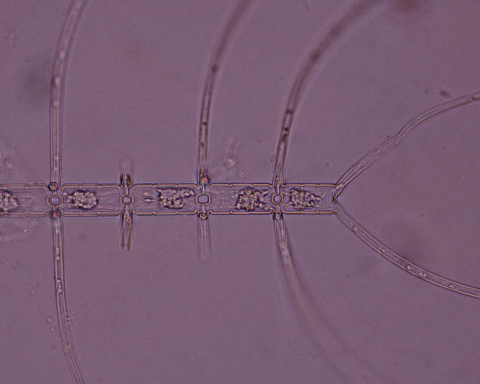
\includegraphics[height=3.6cm]{beifang.png}
    \caption{}
  \end{subfigure}
  \begin{subfigure}{0.3\textwidth}
    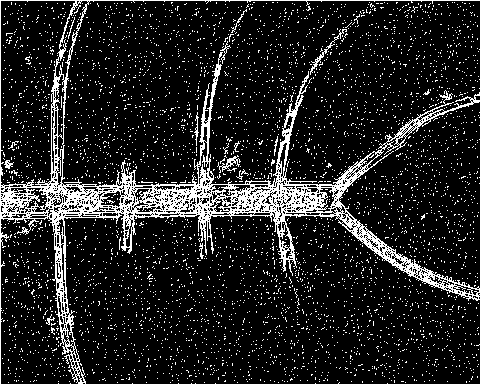
\includegraphics[height=3.6cm]{beifangsvm.png}
    \caption{}
  \end{subfigure}
   \begin{subfigure}{0.3\textwidth}
    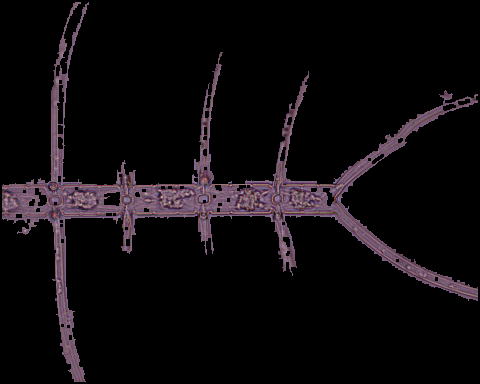
\includegraphics[height=3.6cm]{beifangresult.png}
    \caption{}
  \end{subfigure}
  \\
   \begin{subfigure}{0.3\textwidth}
    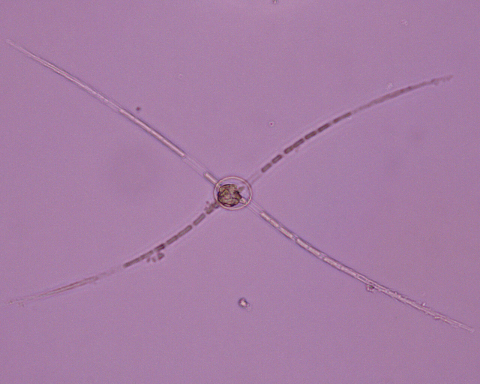
\includegraphics[height=3.6cm]{danmai.png}
    \caption{}
  \end{subfigure}
   \begin{subfigure}{0.3\textwidth}
    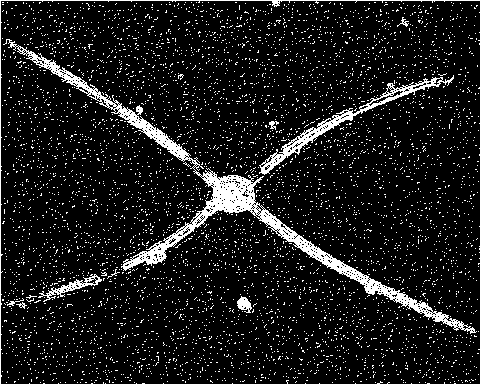
\includegraphics[height=3.6cm]{danmaisvm.png}
    \caption{}
  \end{subfigure}
   \begin{subfigure}{0.3\textwidth}
    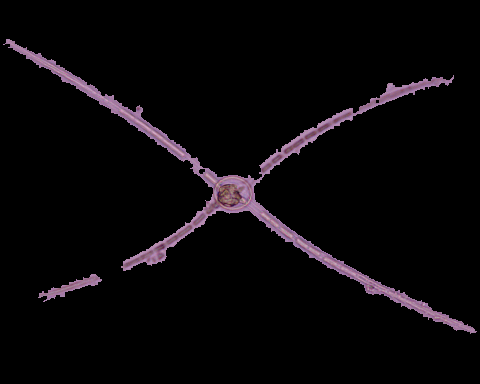
\includegraphics[height=3.6cm]{danmairesult.png}
    \caption{}
  \end{subfigure}
  \caption{支持向量机分类结果和最终分割结果。第一列为原始角毛藻显微图像,第二列为对应的支持向量机分类结果,第三列为采用形态学操作等后续处理过程产生的最终分割结果。}
  \label{svm}
\end{figure}


\section{本章小结}
本章将图像分割问题视为像素分类问题,采用支持向量机对原始图像中的每个像素进行分类。本章详细介绍了支持向量机算法的理论知识和实现过程,然后给出了实验的具体实施步骤以及最终分割结果。实验表明本文的分割方法能够获得较为理想的效果,最终的分割结果可以将图像中复杂的角毛部分较为精确和完整地提取出来。

 

%%% Local Variables: 
%%% mode: latex
%%% TeX-master: t
%%% End: 

\chapter{总结与展望}

\section{总结}
本文针对角毛藻独特的生物形态特征以及其显微图像的特点,提出了一种灰度曲面方向角模型和支持向量机结合的角毛藻显微图像分割方法。本文将分割问题视为分类问题并使用支持向量机来完成分类,所得图像中的所有像素将被分为目标和背景两部分。灰度曲面方向角模型用于产生支持向量机的输入特征,连通域预分割结果用于产生支持向量机的训练样本。经过实验验证,本文的分割方法能够被成功运用在角毛藻显微图像数据集上并且取得了很好的效果。本文的主要内容如下:
\begin{enumerate}
\item 角毛藻显微图像的特征提取,通过分析角毛藻独特的生物形态特征以及显微图像的特点,利用灰度曲面方向角模型实现角毛藻显微图像的特征提取,使用该算法可以有效地提取角毛特征信息,获得比传统特征提取方法更为精确、完整的效果。
\item 连通域预分割,选择所提取特征图中含有较多角毛信息和细胞体边缘信息的两幅灰度特征图进行预分割操作,利用大津法和最大连通域填充处理所选特征图得到预分割结果。
\item 支持向量机分类和后续处理,使用支持向量机进行分类,训练过程中输入灰度映射特征和预分割结果,预测过程中输入原始待处理图像及其对应的特征图。分类结束后,通过选取最大连通域及一些形态学操作处理
分类结果图,最终得到角毛藻显微图像的分割结果。实验结果表明,本文的方法可以较为完整、精确地分割出角毛藻目标细胞及其角毛部分来。
\end{enumerate}
\section{展望}
本文提出的角毛藻显微图像分割的方法能够有效地达到预期的分割效果,但是仍然存在一些需要研究并改进的方面:
\begin{enumerate}
\item 虽然本文的方法可以提取出大量的角毛信息,但是角毛藻轮廓部分仍然存在一些没有填充完整的地方且角毛边缘不平滑,还需要进一步研究和处理。
\item 本文的方法只对单个角毛藻目标细胞分割有效,对于多个角毛藻细胞,无法得到令人满意的效果,需要继续改进和优化方法。
\end{enumerate}

\include{data/chap06}

%%% 其它部分
\backmatter

% 本科生要这几个索引,研究生不要。选择性留下。
\makeatletter
\ifthu@bachelor
  % 插图索引
  \listoffigures
  % 表格索引
  \listoftables
  % 公式索引
  %\listofequations
\fi
\makeatother


% 参考文献
\bibliographystyle{thubib}
\bibliography{ref/refs}


% 致谢
%%% Local Variables:
%%% mode: latex
%%% TeX-master: "../main"
%%% End:

\begin{ack}
转眼间,四年的大学时光已接近尾声。短短四年,使我从一个懵懂无知的孩子变成了一个成熟的青年,对我人生来说是必不可少的经历和体验,虽然短暂快乐的大学生活就要结束了,但这对我来说是一个新的起点、新的开始。回顾这四年,我收获了很多,而这是和一直关心帮助我的人密不可分的。

   首先,感谢我的母校中国海洋大学,这里严谨的学术氛围、优美的校园环境使我这四年的每一天都过的很充实、快乐。

   另外,感谢我的导师郑海永老师对我的帮助和支持,他对科研的热情和进取的学术态度都将对我以后的学习和生活产生影响,很高兴能在未来的三年研究生生活中继续在他的指导下学习和科研。

   此外,感谢我的室友,很荣幸这四年你们一直在我身边。我们一起上课、一起吃饭、一起逛街、一起在考试前挑灯夜战的复习……正因为有你们的陪伴,我才度过了一个美好难忘的大学生活。

   最后,我要感谢我的父母和家人,你们对我的无偿支持和鼓励使我有了保持前进的动力和战胜困难的信心及勇气,使我能够毫无旁骛的专心学业,得以顺利毕业。

   在此,由衷的感谢这些帮助并支持过我的人。


\end{ack}


% 附录
%\begin{appendix}
%%%% Local Variables: 
%%% mode: latex
%%% TeX-master: "../main"
%%% End: 

\chapter{}
\label{}

\chapter{}
\section{}

\chapter{}


%\end{appendix}

% 个人简历
\include{data/resume}
\end{document}
